%\documentclass[aspectratio=169]{beamer}
\documentclass{beamer}
\usetheme{PaloAlto}
%\usetheme{AnnArbor}
\setbeamercovered{transparent}

\usepackage[utf8]{inputenc}

\title{Curso de BEAMER.}
\author[Felipe]{Felipe F. Soares.}
\institute[UFC]{Universidade Federal do Ceará \\ ufc.br}
\date{2016}
%\date{}
%\date{Nome do evento, 2016}
\logo{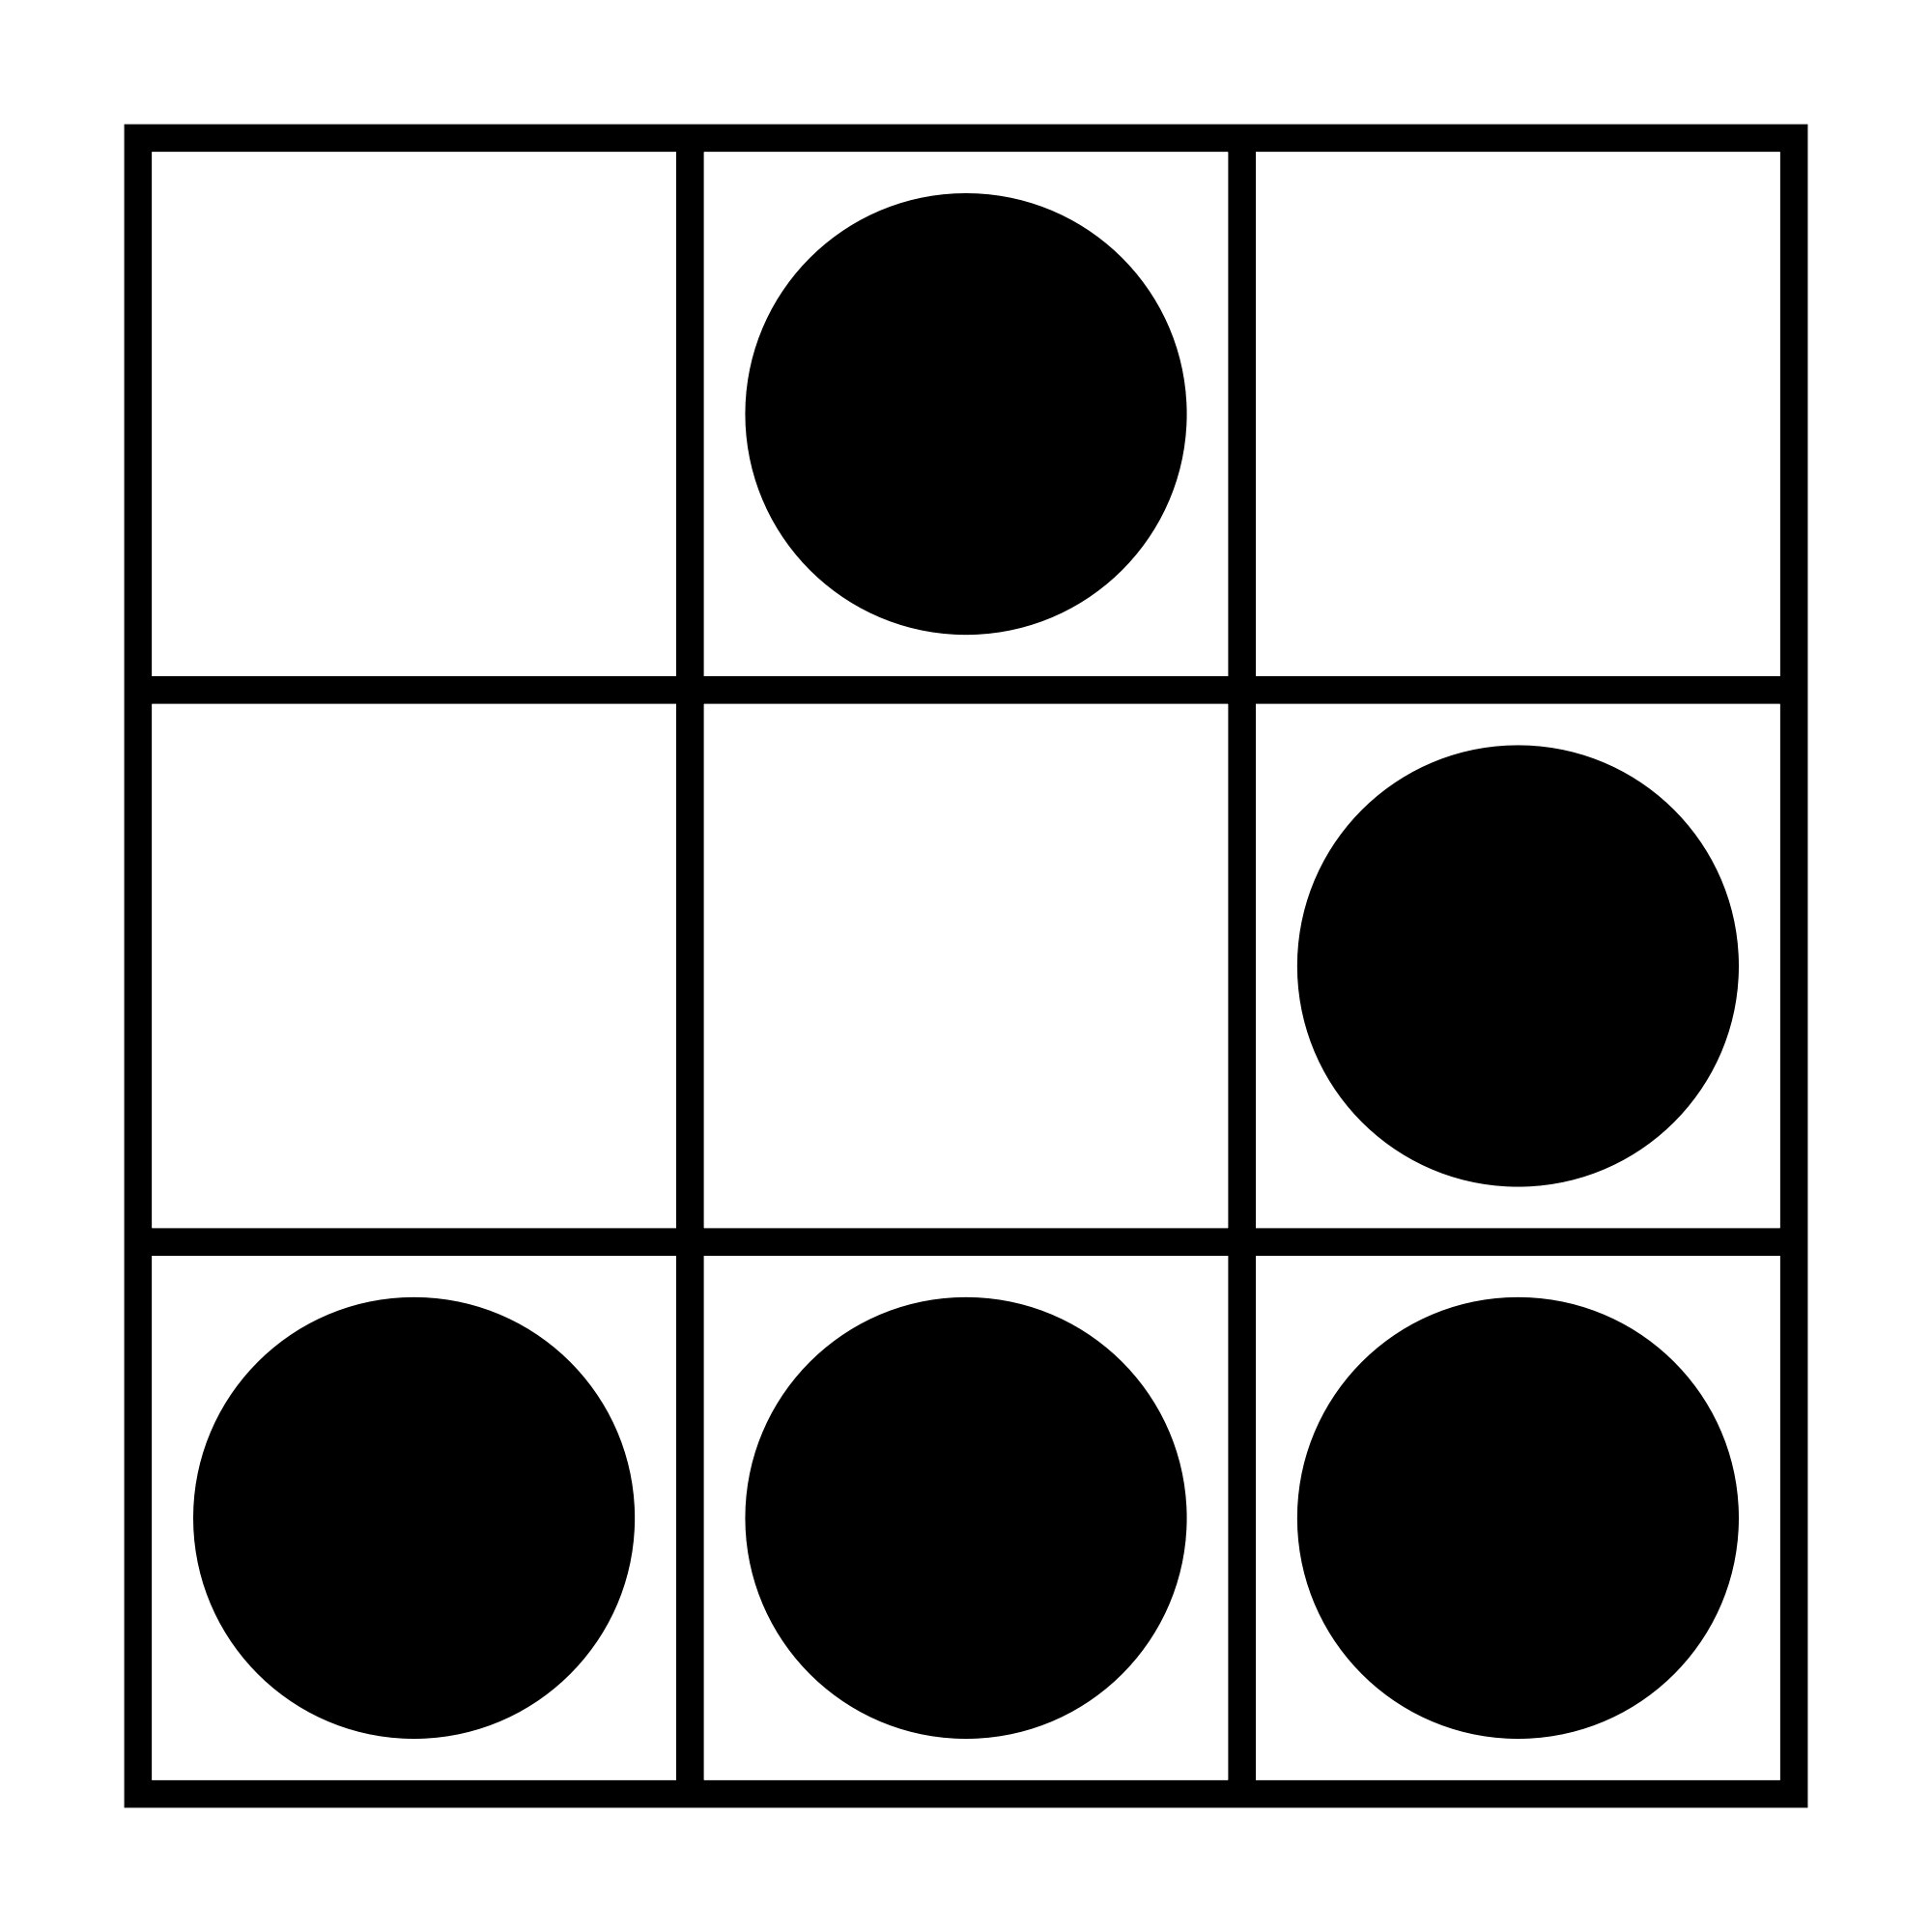
\includegraphics[scale=0.01]{images/glider.png}}

\begin{document}
	\begin{frame}{Esse é o título do quadro}
		\titlepage
	\end{frame}
	
	\begin{frame}
		\frametitle{Esse é o título do quadro uncover}
		\framesubtitle{Esse é o subtítulo}
		
		\uncover<1-3,5>{Vamos resolver uma equação do segundo grau:
		$$ax^2 + bx + c = 0$$ }
		
		\uncover<2->{Primeiro identifique os coeficientes $a$, $b$ e $c$.}
		
		\uncover<3>{Em seguida, calcule o valor de :
		$$\Delta = b^2 - 4ac$$}
		
		\uncover<4->{Calcule a primeira raiz:
		$$x_1 = \frac{-b + \sqrt{\Delta}}{2a}$$}
		
		\uncover<5->{Calcule a segunda raiz:
		$$x_2 = \frac{-b - \sqrt{\Delta}}{2a}$$}
		
	\end{frame}
	
	\begin{frame}
		\frametitle{Esse é o título do quadro visible}
		\framesubtitle{Esse é o subtítulo}
		
		\visible<1>{Vamos resolver uma equação do segundo grau:
		$$ax^2 + bx + c = 0$$ }
		
		\visible<2>{Primeiro identifique os coeficientes $a$, $b$ e $c$.}
		
		\visible<3>{Em seguida, calcule o valor de :
		$$\Delta = b^2 - 4ac$$}
		
		\visible<4>{Calcule a primeira raiz:
		$$x_1 = \frac{-b + \sqrt{\Delta}}{2a}$$}
		
		\visible<5>{Calcule a segunda raiz:
		$$x_2 = \frac{-b - \sqrt{\Delta}}{2a}$$}
		
	\end{frame}
	
	\begin{frame}
		\frametitle{Esse é o título do quadro only}
		\framesubtitle{Esse é o subtítulo}
		
		\only<1>{Vamos resolver uma equação do segundo grau:
		$$ax^2 + bx + c = 0$$ }
		
		\only<2>{Primeiro identifique os coeficientes $a$, $b$ e $c$.}
		
		\only<3>{Em seguida, calcule o valor de :
		$$\Delta = b^2 - 4ac$$}
		
		\only<4>{Calcule a primeira raiz:
		$$x_1 = \frac{-b + \sqrt{\Delta}}{2a}$$}
		
		\only<5>{Calcule a segunda raiz:
		$$x_2 = \frac{-b - \sqrt{\Delta}}{2a}$$}
		
	\end{frame}
	
	\begin{frame}
		\frametitle{Esse é o título do quadro itemize}
		\framesubtitle{Esse é o subtítulo}

		\begin{itemize}				
		
		\item<1- | alert@1-> Vamos resolver uma equação do segundo grau:
		$$ax^2 + bx + c = 0$$ 
		
		\item<2- | alert@2> Primeiro identifique os coeficientes $a$, $b$ e $c$.
		
		\item<3- | alert@4> Em seguida, calcule o valor de :
		$$\Delta = b^2 - 4ac$$
		
		\item<4-> Calcule a primeira raiz:
		$$x_1 = \frac{-b + \sqrt{\Delta}}{2a}$$
		
		\item<5-> Calcule a segunda raiz:
		$$x_2 = \frac{-b - \sqrt{\Delta}}{2a}$$
		
		\end{itemize}
		
	\end{frame}	
	
		\begin{frame}[<+- | alert@+>]
		\frametitle{Esse é o título do quadro itemize}
		\framesubtitle{Esse é o subtítulo}

		\begin{itemize}				
		
		\item Vamos resolver uma equação do segundo grau:
		$$ax^2 + bx + c = 0$$ 
		
		\item Primeiro identifique os coeficientes $a$, $b$ e $c$.
		
		\item Em seguida, calcule o valor de :
		$$\Delta = b^2 - 4ac$$
		
		\item Calcule a primeira raiz:
		$$x_1 = \frac{-b + \sqrt{\Delta}}{2a}$$
		
		\item Calcule a segunda raiz:
		$$x_2 = \frac{-b - \sqrt{\Delta}}{2a}$$
		
		\end{itemize}
		
	\end{frame}	
	
	\begin{frame}
		\frametitle{Esse é o título do quadro - block.}
		\framesubtitle{Esse é o subtitulo do quadro}
		
		\begin{block}<1>{Título}
			Bloco 1
		\end{block}
		
		\begin{block}<2>{Título}
			Bloco 2
		\end{block}
		
		\begin{block}<3>{Título}
			Bloco 3
		\end{block}
		
		\begin{block}<4>{Título}
			Bloco 4
		\end{block}
		
	\end{frame}
	
	
	\begin{frame}
		\frametitle{Esse é o título do quadro - figure.}
		\framesubtitle{Esse é o subtitulo do quadro}
		
		Aqui vem um texto		
		\begin{figure}
			\centering
			\includegraphics<1>[scale=0.01]{images/glider.png}
			\includegraphics<2>[scale=0.01]{images/glider.png}
			\includegraphics<3>[scale=0.01]{images/glider.png}
			\includegraphics<4>[scale=0.01]{images/glider.png}
		\end{figure}
		
		
	\end{frame}
	
\end{document}